%-----------------------------------------------------------------------------
%
%               Template for sigplanconf LaTeX Class
%
% Name:         sigplanconf-template.tex
%
% Purpose:      A template for sigplanconf.cls, which is a LaTeX 2e class
%               file for SIGPLAN conference proceedings.
%
% Author:       Paul C. Anagnostopoulos
%               Windfall Software
%               978 371-2316
%               paul@windfall.com
%
% Created:      15 February 2005
%
%-----------------------------------------------------------------------------


\documentclass[10pt]{sigplanconf}

% The following \documentclass options may be useful:
%
% 10pt          To set in 10-point type instead of 9-point.
% 11pt          To set in 11-point type instead of 9-point.
% authoryear    To obtain author/year citation style instead of numeric.

\usepackage{amsmath}
\usepackage{graphicx}
\usepackage{subfigure}
\usepackage{multirow}
\usepackage{rotating}
\usepackage{array}
%\usepackage{algorithmic}
%\usepackage{algorithm}
\usepackage{textcomp}
\usepackage{listings}
\usepackage{hyperref}
\usepackage{url}
\usepackage{breakurl}
\begin{document}

%\conferenceinfo{SPLASH '11}{date, City.}
%\copyrightyear{2011}
%\copyrightdata{[to be supplied]}

\conferenceinfo{SPLASH'11 Companion,} {October 22--27, 2011, Portland, Oregon,
USA.}
\CopyrightYear{2011}
\copyrightdata{978-1-4503-0942-4/11/10}

\titlebanner{Crossfire Debugging Protocol}        % These are ignored unless
\preprintfooter{Crossfire - Multiprocess, Cross-Browser, Open-Web Debugging Protocol}   % 'preprint' option specified.

\title{Crossfire - Multiprocess, Cross-Browser, Open-Web Debugging Protocol}


\authorinfo{Michael G. Collins}
           {IBM Research - Almaden}
           {mcollins@collinsmichaelg.com}
\authorinfo{John J. Barton}
           {IBM Research - Almaden}
           {johnjbarton@johnjbarton.com}

\maketitle

%\begin{abstract}
We present \textit{Crossfire}, a system and protocol designed to enable
debugging of Web pages in another process or machine. Issues specific to any one
Web browser are abstracted by the protocol and implementation,
allowing a new generation of Open Web development tools to be implemented. We discuss the major refactoring of Firebug, the open source Web debugging tool
to use \textit{Crossfire} and the interplay between goals and resources that such an effort requires.
In addition to the cross-browser focus of the protocol, we also discuss support for extensions which themselves will be
cross-browser and client-server.
\end{abstract}
\begin{abstract}
We present \textit{Crossfire}, a system and protocol designed to enable
debugging of Web pages in another process or machine. Issues specific to any one
Web browser are abstracted by the protocol and implementation,
allowing a new generation of Open Web development tools to be implemented. We discuss the major refactoring of Firebug, the open source Web debugging tool
to use \textit{Crossfire} and the interplay between goals and resources that such an effort requires.
In addition to the cross-browser focus of the protocol, we also discuss support for extensions which themselves will be
cross-browser and client-server.
\end{abstract}

\category{  D.2.5}{Software Engineering}{Testing and Debugging— debugging aids, distributed debugging}


\terms
Experimentation, Reliability

\keywords
Source-Level Debugging, Distributed Debugging, Open Source


\section{Introduction}
Web Applications continue to grow in size and complexity. Asynchronous background 
data download (AJAX) started the surge. 
This led to the 
emergence of common toolkits and libraries for Javascript which drove  performance
increases in Web Browsers fueling more growth in client-side Web application
development. These improvements, combined with new features available in Web browsers 
shifted investment from server- to client-side. Recent empirical analysis of representative
 major Web sites shows program sizes in the range of hundreds of kilobytes of
sophisticated code.\cite{VitekDynamicJS2010}

To develop and maintain these large applications, programmers and designers rely on 
numerous tools, most notably Web page debuggers. 
This paper describes a major re-architecting of the most widely used Web page debugger, 
Firebug, as a client/server system and in particular the 
\textit{Crossfire} protocol designed to support its client-server communications.  
Our description focuses on practical, state-of-the-art issues in an on-going and fast-moving project. 
Thus we cover details of protocol important for implementation and issues of 
matching resources to goals important for project management: we must deal with both 
extremes to succeed.

\section{Background}
To understand the importance and challenges of the \textit{Crossfire} work we start by introducing Firebug.
Released by Joe Hewitt in 2006, Firebug was the first integrated Web debugger. Firebug is a runtime 
debugger: it directly accesses, responds to, and operates on the running Web browser.  Rather than separate 
views of JavaScript, CSS, and HTML, Firebug integrated its views such that interaction with, 
for example, an HTML element would cause synchronized views of the CSS rules. Rather than static 
 views of browser state, Firebug included dynamics like network traffic analysis and console logging; rather 
than read-only views, Firebug allowed live edits where possible so developers could try out changes.
The resulting tool became very popular with developers and contributing significantly to the growth in Web applications.

The primary implementation of Firebug is a Firefox extensions, a supplemental software 
component that loads into the Firefox Web browser. A secondard implementation with fewer features and, 
in particular, limited support for JavaScript debugging, called Firebug Lite works in multiple browsers. 
The success of Firebug lead to implemenations of Web Page debuggers in other browsers, including 
DragonFly for Opera, Web Inspector for Google Chrome and Apple Safari, and the developer tool in 
Microsoft Internet Explorer. Since 2007 Firebug has been developed as an open source project, with 
seven major releases.

To give a flavor of the kinds of operations Firebug supports, we outline two examples more completely
described in Ref.\cite{jjb-www2010}. First suppose a developer wants to understand why a block of text 
in the Web page turned green while the page was loading. More. 

Second, 

(Refactoring timeline)
\input{design.tex}
\section {Crossfire}

The Crossfire protocol is an asynchronous, bi-directional protocol designed to
enable the full functionality of the Firebug debugger in a multi-process or
remote scenario. Where it was possible, the design of the protocol took cues
from existing debug protocols such as DBGP\cite{dbgp}, Opera
Scope\cite{opera-scope}, Google's Chrome Dev Tools\cite{chrome-dev-tools} , as
well as common Web technologies (e.g. HTTP, JSON\cite{json}). Certain
features unique to Firebug and to debugging code running inside a Web Browser
had to be taken into account in the design of the protocol.
We give an overview of the protocol and discuss some aspects that are important to its design.

\subsection {Overview}
Debugging the code that implements a Web page or Web application differs in some
significant ways from debugging applications developed for other types of
systems. HTML and CSS are used to declaratively specify the structure and style of the
user-interface, which is rendered by the Web browser. Developers cannot (easily)
debug the rendering code itself. Instead, built-in tools like Firebug allow the
developers to interact with the rendering engine by modifying the input and
observing the output in real time, via live CSS and DOM editing. JavaScript code
on the page can be stepped through when it is executing, however there is no
guarantee that any JavaScript code is necessarily running at any given moment.
JavaScript code on a Web page can be triggered by timers, user interactions or
network events. There is no outermost main or idle loop to return to; when a
section of JavaScript code is finished executing, control returns to the Web
browser. This confounds attempts at things such as a simple 'halt' command,
which is common among debuggers for other systems. The closest analog in Firebug
is the \textit{break-on-next} feature.

The Crossfire protocol is heavily event-driven, and requests made via Crossfire
are asynchronous. This differs from many other debug protocols which are often
synchronous or a combination of synchronous and asynchronous calls.  The reasons
for this decision stem from the nature of code running in a web page, and the
fact that in some scenarios, especially the intermediate scenarios we wished to
achieve, we would have a remote client connected to a server which also had a
co-resident debug UI (Firebug). In other words, a complete Firebug and Crossfire
server implementation would be running in a single Firefox process, and clients
could connect to the Crossfire server. The result of this scenario is that
clients cannot assume or rely on being the only agent acting on the runtime
engine. For instance, a Crossfire client cannot safely assume that the debugger
will remain suspended on a line of code until the client issues a request to
resume. It is also possible that this action was triggered by the user from
another client (in this case it is helpful to think of Firebug's in-process UI
as another client to the debugger). However any connected Crossfire client will
receive an event whenever the JavaScript debugger suspends or resumes, and
should react accordingly.

Implementations of the protocol differ based on whether the implementation is
intended to operate as a client or server. A Crossfire server resides in or is
connected to the process which is acting as the runtime platform for the Web
page, application, or other code which is to be debugged. This is typically a
Web Browser, although supporting other runtime environments is envisioned. A
Crossfire client connects to a server in order to receive events and issue
requests, typically in order to provide a user-interface
for debugging, (e.g. GUI or command-line debugger). It is not necessary for the
client and server to reside in the same process or even the same host machine.



%\begin{figure}[htp]
%  \includegraphics  [width = 86 mm] {figures/crossfire-example-packet.png}
%  \caption{An example of a Crossfire message packet.}
% \label{fig:crossfire-packet}
%\end{figure}
% \texttt{
% Content-Length:219
% \\r\\n\\r\\n
% {
%   "type":"request",
%   "command":"setbreakpoint",
%   "context_id":"http://localhost:8080/test.html",
%   "seq":21,
%   "arguments": {
%                  "position":0,
%                  "enabled":true,
%                  "target":"http://localhost:8080/test/some_javascript.js",
%                  "line":9,
%                  "ignoreCount":0,
%                  "type":"line"
%                }
% }
%\\r\\n
%}
\subsection {Connection and Handshake}
To avoid conflicts with existing ports,
Crossfire does not specify a standard or well-known port. Port agreement is left
up to the user, or the client software must start the server listening on
the same port it will attempt to connect to.

The connection protocol is purposefully conventional.
The Crossfire server listens for a TCP connection on the specified port (greater
than 1024).  A client wishing to connect sends the string ``CrossfireHandshake''
followed by a CRLF (a blank line specified by a carriage-return followed by a
line-feed character, as with HTTP). An optional second handshake line may
contain a comma-separated list of tool names to be enabled immediately, followed
by another CRLF. The server replies with the same handshake string, at which
point the connection is established and the client may begin sending requests and
receiving events from the server.

\subsection {Client/Server Behavior}
Once a connection has been established and a successful handshake is completed,
the server may begin sending events to the connected client using the same TCP
connection used for the handshake. A client may also begin sending requests to
the server using the same connection. Clients should not expect the server to
respond synchronously to requests or in order. The most common example is a
Crossfire server sending one or more events to the client before responding to a
client's request, because the events occurred during the time the request was
being sent or processed.

\subsection {Message Packets}
As described above, the packet format follows the design of the Google Chrome browser\cite{V8}.
A well-formed Crossfire packet contains one or more headers consisting of the
header name, followed by a colon (``:``), the header value, and terminated by a
CRLF. A ``Content-Length'' header containing the number of characters in the
message body is required, and additional headers are allowed.

The message body is separated from the headers by another CRLF blank line.
The blank line is followed by a well-formed JSON string. The message must contain a ``type'' field with the value one of
``request'', ``response'', or ``event'', and a ``seq'' field which contains the
sequence number of the packet. The sequence number of each message should
be greater than that of the last message received.

\subsection {Contexts}
Unlike desktop or server application debuggers, a Web browser typically runs
multiple applications or Web pages. A developer is likely to debug one or two of these applications,
while the rest are unrelated to the application. The debugger must
have a mechanism to focus on the particular page being debugged.
Firebug represents an instance of a Web page via an object called a
\textit{Context}. The context object allows Firebug's panels and modules to
share information about a web page that is being debugged, therefore it has a
central role in Firebug's architecture.

Most of the events that occur in a Web browser that are of interest to a debug
UI are related to individual pages, and therefore individual Firebug contexts.
Examples of context-specific events include loading (or reloading) of a page,
loading and compiling a script, errors being generated from an executing script,
DOM elements being added or modified, a breakpoint being added to a script, etc.

The Crossfire protocol uses contexts for
most requests / events. Crossfire represents a context as a mapping of the
unique context ID and the URL of the page. This allows a connected Crossfire
client to distinguish between separate loads of the same URL, as is often the
case when a developer reloads a page several times in the course of developing
or debugging the page.
Firebug's TabWatcher component monitors loading and unloading of Firefox windows
and tabs.  The Crossfire server assigns a unique identifier to each
context, and passes this ID as part of most event and response packets.

\subsection {Breakpoints}
Breakpoint debugging is a standard tool for debugging software at runtime in
many languages and environments. The Web Browser environment creates several
challenges for designing a remote protocol which supports breakpoint debugging.
Firebug also introduces several types of breakpoints which are not present in
other environments \cite{jjb-www2010}.

Even the simplest case, a JavaScript line breakpoint, has design implications
that must be considered. Typically, such a breakpoint is identified by a line
number and the URL of the script. However, existing JavaScript debugging APIs
such as Firefox's do not contain the concept of Firebug's contexts.  Therefore
if a user places a breakpoint on line 23 of a URL http://localhost/script.js,
then that breakpoint will exist for all occurrences of that URL. This may or may
not be what the user actually desires.  Considering the increasing use of
JavaScript libraries, it is entirely likely that a script from the same URL is
loaded into two completely unrelated pages. It is conceivable that a user would
wish to debug his or her code and the interaction with the library, without
affecting code running in another tab or window.

Crossfire's breakpoint protocol allows breakpoints to be set in one of two ways,
either with or without a context ID. If a Crossfire client specifies a context
ID along with a request to set a breakpoint, then that breakpoint should be
enabled for that location in any existing context, or a future context which is
created with the same URL in the same container (i.e. the page is reloaded).

If a client does not specify a context (by passing null as the value of the
context ID), then the behavior is to set a breakpoint for the specified location
in any future contexts. The intended use case for this behavior is setting a
breakpoint in a client UI such as an editor, where the source code location has
changed (due to editing), but the changes have not yet been applied to the page
in the browser.

More advanced breakpoints, such as the HTML element breakpoints, are supported
by specifying that the \textit{location} property of a breakpoint in Crossfire
is an arbitrary JSON object. A location object is defined depending on
the type of breakpoint.  A JavaScript line breakpoint has a location object
which consists of a target URL and line number. Firebug's HTML breakpoints have
a location object which consists of an XPath expression that identifies the
target element.  Eventually other location types may be added, e.g. to support
network-related breakpoints such as Firebug's \textit{Break-On-XHR} feature.

\subsection {Extensibility}
One of the goals of Crossfire is to support remote and multi-process versions of
Firebug. One of Firebug's features is its ability to be extended, and there are
already many existing extensions. Therefore, we have developed what an API for
Crossfire, called the \textit{Crossfire Tools API}. The Tools API allows Firebug
extension developers a clean and consistent way to access the Crossfire client
and/or server connection.

On the server-side, the Tools API allows an extension to send custom events
and handle custom requests using Crossfire's connection and transport mechanism.
A client extension can listen for these events and respond to the requests.
Using this API, it will be possible for Firebug extensions to continue to adapt
to architectural changes in future versions of Firebug.

One consequence of this design choice is that the set of possible commands or
event names cannot be specified definitively by the protocol. A Crossfire
client or server must therefore be able to accept and respond to any well-formed
message packet, even if it may not know how to handle a particular command or
event type.

\section{Implementation}

\subsection{Crossfire Firefox Extension}
The first implementation of the Crossfire protocol is an extension implements
the protocol as an extension to Firefox and Firebug. The extension is
implemented entirely in JavaScript, using a modular design to allow us to share
code between client and server implementations, as well as cross-browser
implementations. This extension implements a flexible transport layer, allowing
the extension to operate as either a Crossfire client or server. This will also
enable both client and server to be implemented on top of other transport
layers, such as Web Sockets or HTTP.

The extension can be started in client or server mode either from the Firefox
user interface, or via command-line switches to Firefox. This latter mode of
operation allows external tools to launch Firefox and start the Crossfire server
listening on a known port so that the external tool may automatically connect
back to it. Figure \ref{fig:crossfire-arch}

In order to support Firebug's ability to operate both in-process and
out-of-process, an asynchronous API which we called BrowserToolsInterface was
put in place to broker calls between Firebug's front- and back-end pieces.

\subsection{Crossfire Tools API}
The Crossfire extension also implements an API, called the ``Crossfire Tools
API'' which enables extensibility of the Crossfire system and protocol. Firebug
features such as the Console, Inspector, and Net Panel, are implemented as tools
using the API, allowing them to be enabled/disabled independently.

A tool can be implemented as a JavaScript file or collection of files that
implements the Crossfire Tools API. The tool registers itself with the core
Crossfire Module, providing an identification string that is used to identify
messages via the 'tool' header. In server operation, the tool is then able to
receive notification when a connection is created or when request packets are
received. The Tools API allows a tool to access Crossfire's transport layer in
order to send events or command responses.  Typically, a tool operating within
the context of a Crossfire server might register listeners with one or more
Firebug modules, in order to dispatch events generated by the module to the
remote connection. A tool operating as part of a Crossfire client would process
the events sent from the server tool, and update part of the client UI, such as
a Firebug panel. The tool could also listen for client events from the UI, and
send the appropriate requests to the server, to be handled by the tool's
server-side component.

\begin{figure}[htp]
  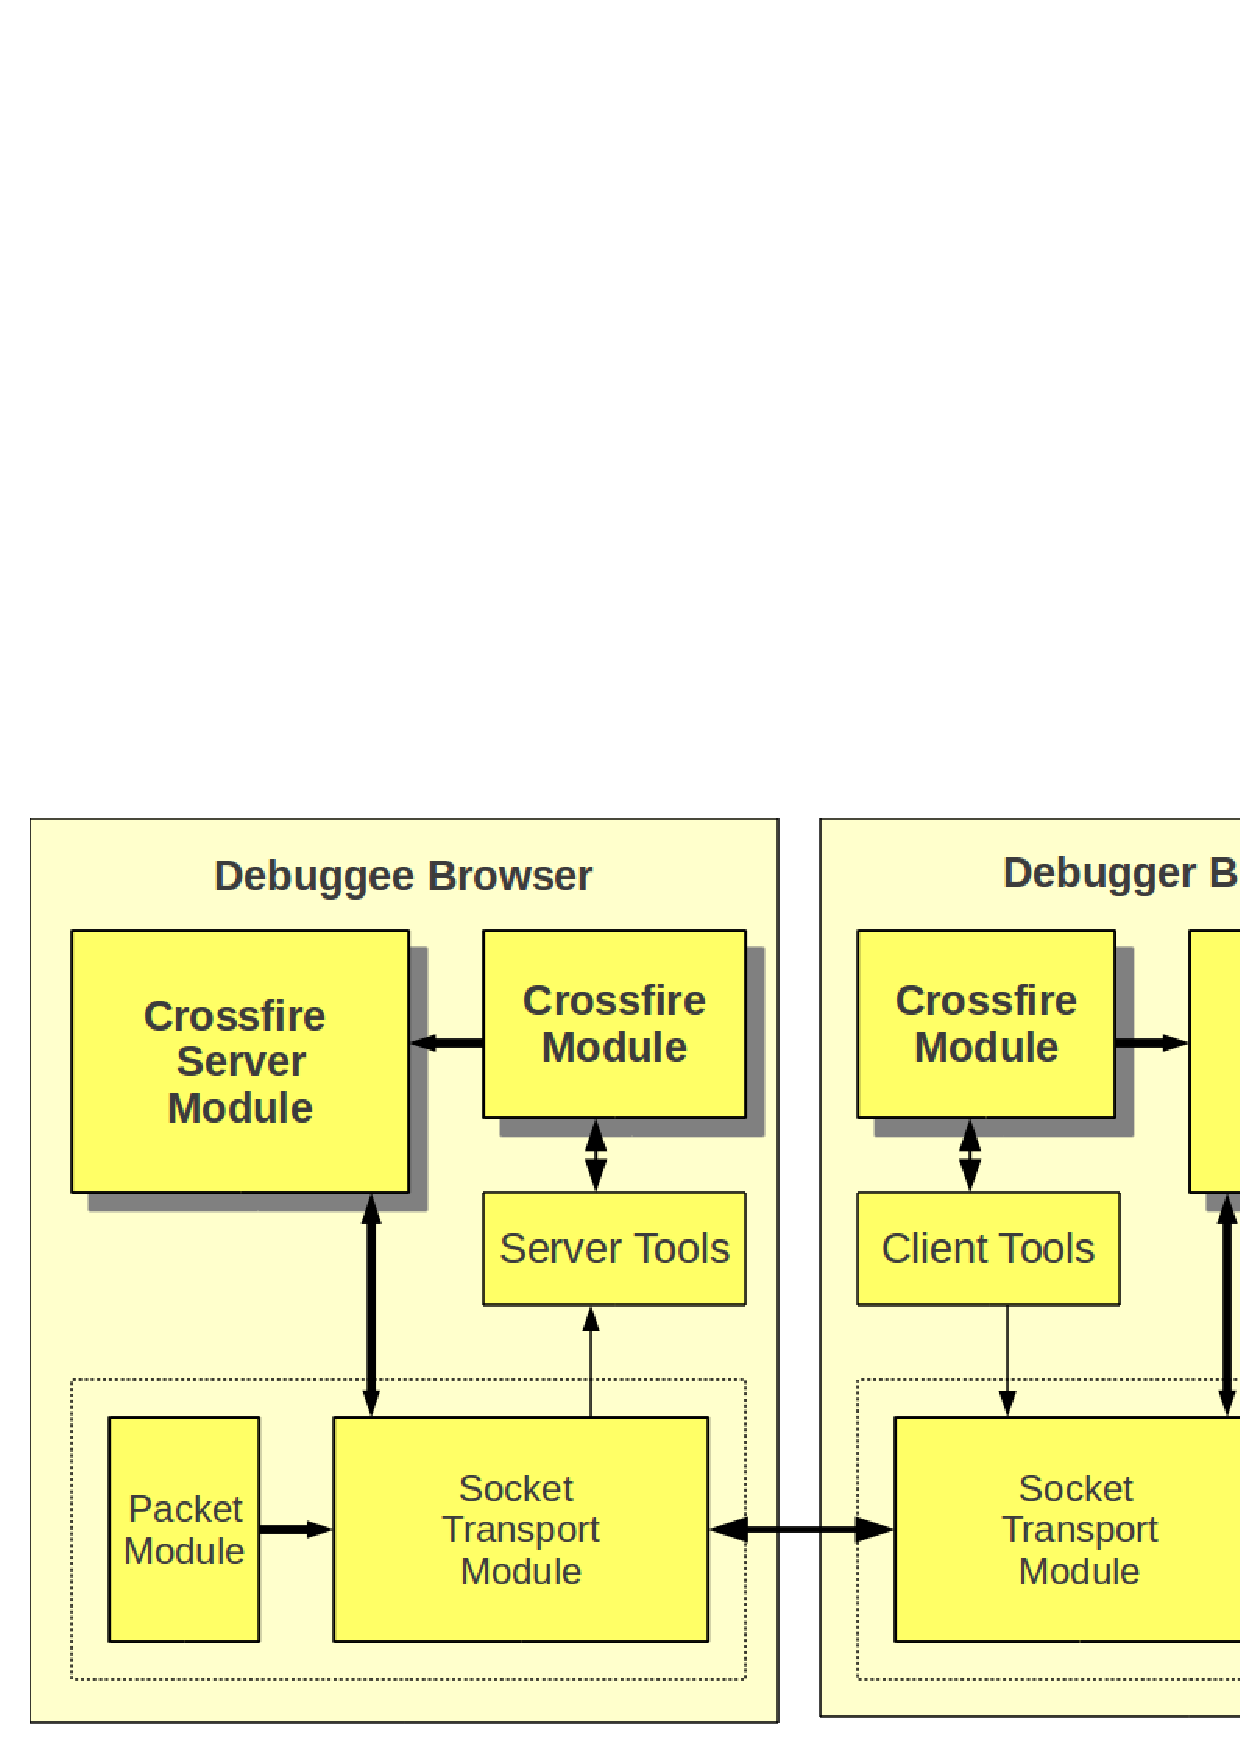
\includegraphics  [width = 86 mm] {figures/crossfire-arch4.png}
  \caption{Crossfire Firefox Extension Architecture}
 \label{fig:crossfire-arch}
\end{figure}

\subsection{Modules}

\subsection {Browser Tools Interface}

\section{Related Work}
\subsection{Web Development Tools}
\subsubsection{Internet Explorer}
\subsubsection{Chrome Dev Tools}
\subsubsection{Wienre}
\subsubsection{Eclipse JSDI}
\subsubsection{Orion}
\subsection{Remote Protocols}
Many protocols have already been designed for the purposes of remotely debugging
an application running in another process, virtual machine, host, etc. The GNU
GDB debugger has an associated Remote Serial Protocol (RSP)\cite{gdb-rsp}. While
it is the only debugger we know of with its own song \cite{gdb-song}, it is
primarily designed for debugging code running on embedded systems, and would not be
well-suited for use with Firebug.
\subsubsection{JNDI/JDWP}
Java does remote debugging too.
\subsubsection{DBGp}
DBGp\cite{dbgp}, is an acronym for Debug Protocol, and was developed for version
2 of the XDebug debugger for the PHP language. Although it was designed not to
be language specific, many of the commands are intended to be synchronous, as
opposed to the asynchronous nature of Crossfire. DBGp also allows for the
debugger engine to send an event to a client via the 'notification' element,
with a custom body. However in order to support Firebug, we would need to define
the same events defined by Crossfire as DBGp notifications.
\subsubsection{Opera Scope Protocol}
The Opera browser has a built-in Web development tool called DragonFly,
which also supports the Scope remote debug protocol. The Scope protocol supports
XML and JSON formats, and features such as JavaScript debugging and remote DOM
inspection.
\cite{opera-scope}


\section {Future Work}
\subsection {Web Sockets}
\subsection {Multi-user Debugging}
\section{Conclusion}
Our work thus far has demonstrated that it is possible to incrementally refactor
and rearchitect an existing codebase while maintaining the ability to support
Firebug's large user-base with releases which are compatible with new releases
of Firefox. In addition we have shown it is possible to implement a system for
remote debugging similar to existing solutions in other browsers, but using a
modular approach that is written purely in JavaScript. The project has been
successful in attracting new contributors and new opportunities for Firebug,
enabling the project to explore new directions. Continuing this work will
provide numerous benefits for Firebug users as well new features that are in
demand, while allowing Firebug to adapt to possible future changes in Firefox,
and increasing the features offered by Firebug/Firebug Lite in other Web
browsers.

Crossfire is an on-going open source project with source\cite{crossfire-src}
and documentation\cite{crossfire-doc} made available as part of the Firebug
project, as is Firebug's source\cite{firebug-src} and developer
documentation\cite{firebug-doc}. Documentation and downloads for Firebug are
also available from the Firebug project's website.\cite{getfirebug}



\acks
As a multi-year open source effort, \textit{Crossfire} results from a broad collaboration and
contributions from many individuals. Simon Kaegi from the Orion team lead us towards collaboration with the Orion and Eclipse teams. Darin Wright wrote the initial implementation of the Tools Interface. Grant Gayed and Mike Rennie heavily influenced the \textit{Crossfire} protocol during their implementation of the IE server and Eclipse clients. Pedro Simonetti Garcia, Kevin Dangoor, and Atul Varma provided key insights to the module loading work. Jan 'Honza' Odvarko powers the Firebug project essential to our evolution strategy, especially implementing a test suite critical to maintaining the quality of the waypoint implementations. Steven Roussey helped with an early implementation and feedback on issues it raised.


% We recommend abbrvnat bibliography style.

\bibliographystyle{abbrvnat}

%\bibliography{bibliography}

% The bibliography should be embedded for final submission.

\begin{thebibliography}{27}
\providecommand{\natexlab}[1]{#1}
\providecommand{\url}[1]{\texttt{#1}}
\expandafter\ifx\csname urlstyle\endcsname\relax
  \providecommand{\doi}[1]{doi: #1}\else
  \providecommand{\doi}{doi: \begingroup \urlstyle{rm}\Url}\fi

\bibitem[web(2001)]{websocketapi}
Web{S}ocket {API} {S}pecification, 2001.
\newblock \url{http://dev.w3.org/html5/websockets/}.

\bibitem[jdw(2004)]{jdwp}
\emph{Java {P}latform {D}ebugger {A}rchitecture}, 2004.
\newblock \url{http://download.oracle.com/javase/1.5.0/docs/guide/jpda/}.

\bibitem[gdb(2007)]{gdb-song}
{GDB} {S}ong, 2007.
\newblock \url{http://www.gnu.org/music/gdb-song.html}.

\bibitem[chr(2009)]{chrome-dev-tools}
Google {C}hrome {D}ev {T}ools {P}rotocol, 2009.
\newblock
  \url{http://code.google.com/p/chromedevtools/wiki/ChromeDevToolsProtocol}.

\bibitem[Web(2010)]{WebInspector}
Web{K}it {W}eb {I}nspector, 2010.
\newblock \url{http://trac.webkit.org/wiki/WebInspector}.

\bibitem[clo(2010)]{cloud9}
Cloud 9, 2010.
\newblock \url{http://cloud9ide.com/}.

\bibitem[gdb(2010)]{gdb-rsp}
\emph{{GNU} {D}ebugger ({GDB}) {M}anual}, 2010.
\newblock \url{http://sourceware.org/gdb/current/onlinedocs/gdb/}.

\bibitem[ope(2010)]{opera-scope}
Opera {S}cope {P}rotocol, 2010.
\newblock \url{http://dragonfly.opera.com/app/scope-interface/}.

\bibitem[web(2010)]{websocketprotocol}
Web{S}ocket {P}rotocol, 2010.
\newblock \url{http://www.whatwg.org/specs/web-socket-protocol/}.

\bibitem[Ecl(2011)]{EclipseJSDT}
Eclipse {JSDT}, 2011.
\newblock \url{http://wiki.eclipse.org/JSDT/Debug}.

\bibitem[Goo(2011)]{GoogleChrome}
Google {C}hrome, 2011.
\newblock \url{http://www.google.com/chrome}.

\bibitem[IET(2011)]{IETools}
Microsoft {I}nternet {Explorer} {D}eveloper {T}ools, 2011.
\newblock \protect\url{http://msdn.microsoft.com/en-us/library/dd565628}.

\bibitem[V8(2011)]{V8}
V8 {D}ebug {P}rotocol, 2011.
\newblock \url{http://code.google.com/p/v8/wiki/DebuggerProtocol}.

\bibitem[com(2011)]{commonjs}
Common{JS}, 2011.
\newblock \url{http://www.commonjs.org/}.

\bibitem[cro(2011{\natexlab{a}})]{crossfire-doc}
Crossfire online documentation, 2011{\natexlab{a}}.
\newblock \url{http://getfirebug.com/wiki/index.php/Crossfire}.

\bibitem[cro(2011{\natexlab{b}})]{crossfire-src}
Crossfire source repository, 2011{\natexlab{b}}.
\newblock \url{http://fbug.googlecode.com/svn/extensions/crossfire/branches/}.

\bibitem[fir(2011{\natexlab{a}})]{firebug-doc}
Firebug developer api documentation, 2011{\natexlab{a}}.
\newblock \url{http://getfirebug.com/developer/api/firebug1.7/}.

\bibitem[fir(2011{\natexlab{b}})]{firebug-src}
Firebug source repository, 2011{\natexlab{b}}.
\newblock \url{http://fbug.googlecode.com/svn/branches/}.

\bibitem[get(2011)]{getfirebug}
Firebug website, 2011.
\newblock \url{http://getfirebug.com}.

\bibitem[ope(2011)]{opera-dragonfly}
Opera {D}ragon{F}ly, 2011.
\newblock \url{http://www.opera.com/dragonfly/}.

\vfill\eject

\bibitem[ori(2011)]{orion}
Orion, 2011.
\newblock \url{http://www.eclipse.org/orion/}.

\bibitem[Barton and Odvarko(2010)]{jjb-www2010}
J.~J. Barton and J.~Odvarko.
\newblock Dynamic and graphical web page breakpoints.
\newblock In \emph{Proceedings of the 19th international conference on World
  wide web}, WWW '10, pages 81--90, New York, NY, USA, 2010. ACM.
\newblock ISBN 978-1-60558-799-8.
\newblock \doi{http://doi.acm.org/10.1145/1772690.1772700}.
\newblock URL \url{http://doi.acm.org/10.1145/1772690.1772700}.

\bibitem[Burke(2011)]{requirejs}
J.~Burke.
\newblock Require{JS}, 2011.
\newblock \url{http://requirejs.org/}.

\bibitem[Caraveo and Rethans(2007)]{dbgp}
S.~Caraveo and D.~Rethans.
\newblock {DBGP, A common debugger protocol for languages and debugger UI
  communication, Draft 16}, 2007.
\newblock \url{http://www.xdebug.org/docs-dbgp.php}.

\bibitem[Crockford(2006)]{json}
D.~Crockford.
\newblock {JSON}, 2006.
\newblock \url{http://json.org}.

\bibitem[Mueller(2011)]{weinre}
P.~Mueller.
\newblock Weinre, 2011.
\newblock \url{http://pmuellr.github.com/weinre/ }.

\bibitem[Richards et~al.(2010)Richards, Lebresne, Burg, and
  Vitek]{VitekDynamicJS2010}
G.~Richards, S.~Lebresne, B.~Burg, and J.~Vitek.
\newblock An analysis of the dynamic behavior of javascript programs.
\newblock In \emph{Proceedings of the 2010 ACM SIGPLAN conference on
  Programming language design and implementation}, PLDI '10, pages 1--12, New
  York, NY, USA, 2010. ACM.
\newblock ISBN 978-1-4503-0019-3.
\newblock \doi{http://doi.acm.org/10.1145/1806596.1806598}.
\newblock URL \url{http://doi.acm.org/10.1145/1806596.1806598}.

\end{thebibliography}

\end{document}
